\section{Track slopes}
\label{sec:slopesmva}
%
An MVA approach was also used to parameterize the uncertainty on the
track slopes. Again the \textbf{BDTG} method from the \textbf{TMVA}
package was used. The input variables were $p$, $\eta$, $\pt$, $\phi$,
$tx$ and $ty$. The highest ranked variables are $p$, $\eta$ and $\phi$
in that order. For training the signal tracks from the virtual photon
$\chicone \rightarrow J/\psi \mu^+ \mu^-$ sample are used. Separate
BDTs are trained for the uncertainites in $tx$ and $ty$.

Figure \ref{fig:coreltx} (Figure \ref{fig:corelty}) shows the correlation between the track fit and emulated
value of uncertainty the relative differecne on $tx$ ($ty$). The
distributions of the fit and emulated values are shown in Fig. ~\ref{fig:etxty}. The fitted
and emulated values agree at the level of $10 \%$ with some
tail. Comparisons of the emulated and fit values of $p$, $\phi$ and
$\eta$ are given in Appendix~\ref{sec:slopeplots}. 
%
\begin{figure}[h!]
\centering
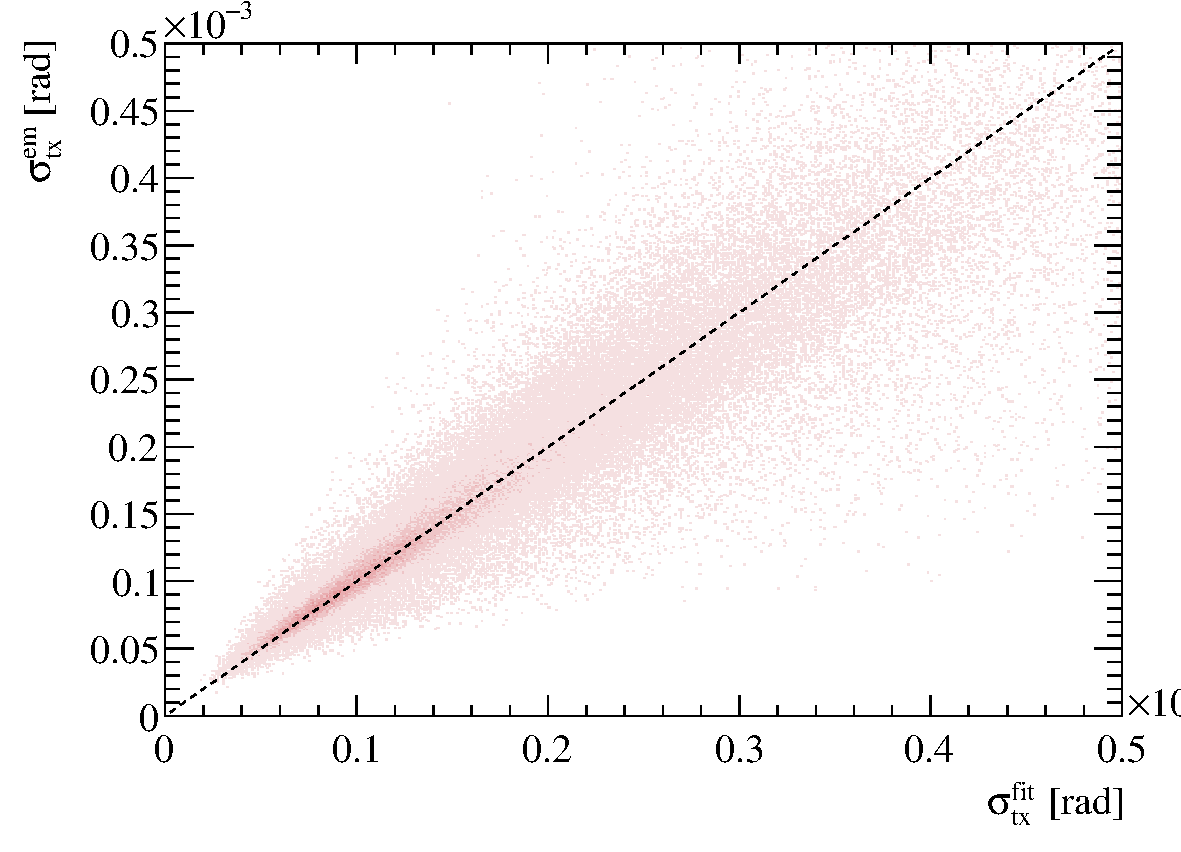
\includegraphics[width=0.48\textwidth]{figs/corelation-tx.pdf}
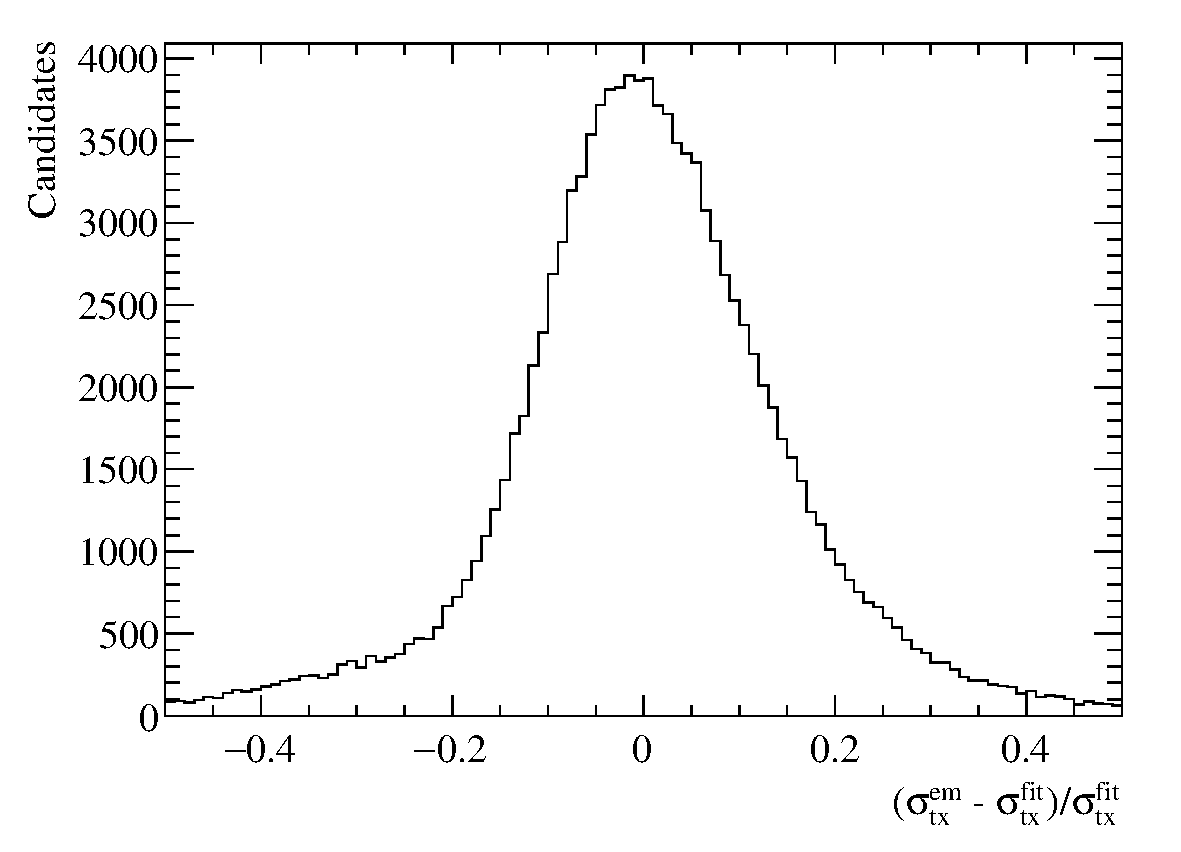
\includegraphics[width=0.48\textwidth]{figs/difference-tx.pdf}
\caption{(Left)  $\sigma^{em}_{tx}$  versus  $\sigma^{fit}_{tx}$. The dotted line
  corresponds to perfect corelation. (Right) Relative difference
  between $\sigma^{em}_{tx}$  and  $\sigma^{fit}_{tx}$.}
\label{fig:coreltx}
\end{figure}
%
%
\begin{figure}[h!]
\centering
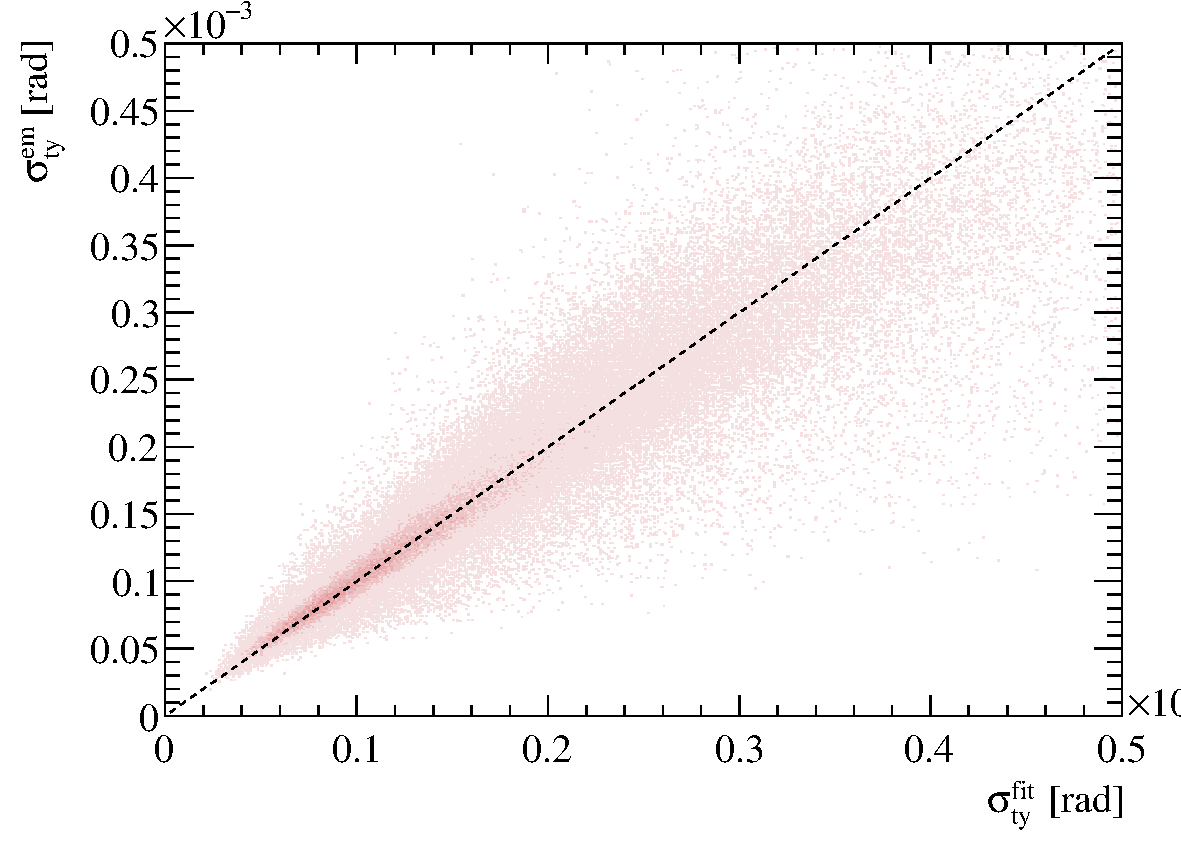
\includegraphics[width=0.48\textwidth]{figs/corelation-ty.pdf}
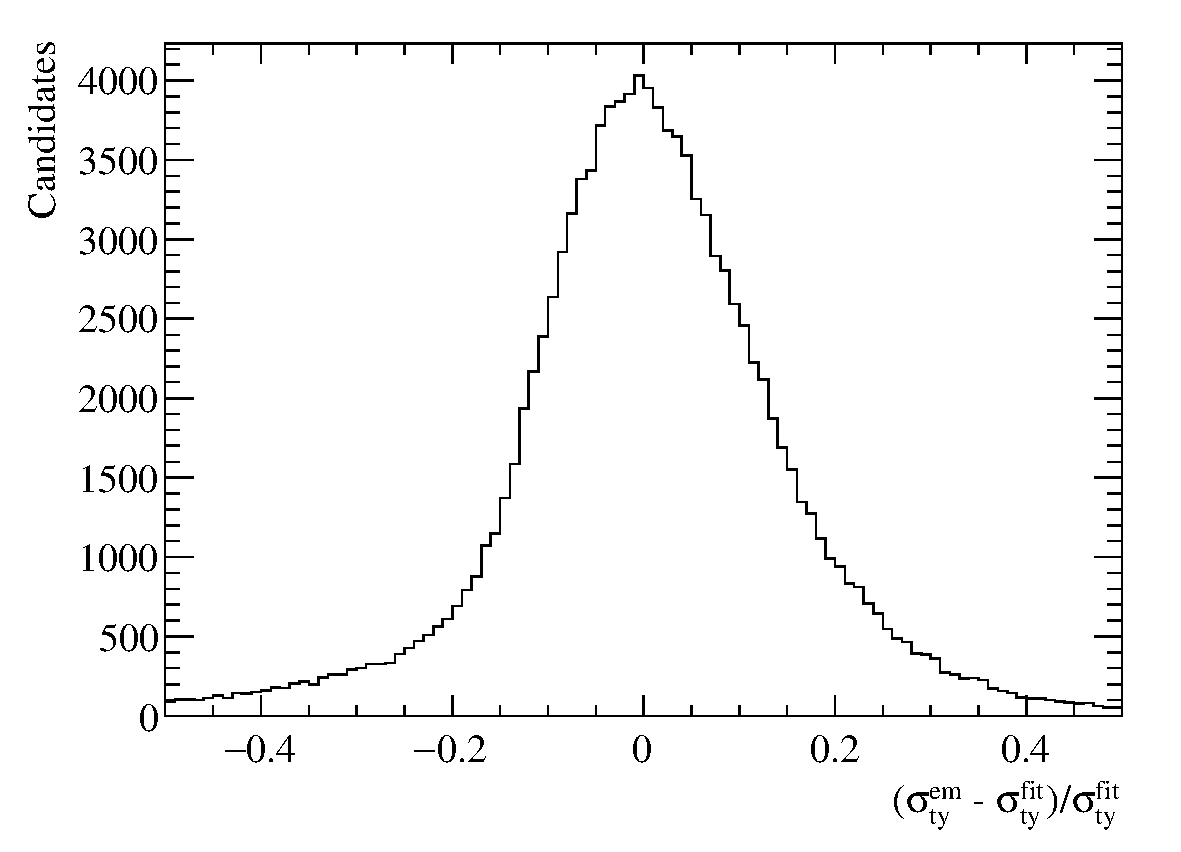
\includegraphics[width=0.48\textwidth]{figs/difference-ty.pdf}
\caption{(Left)  $\sigma^{em}_{ty}$  versus  $\sigma^{fit}_{ty}$. The dotted line
  corresponds to perfect corelation. (Right) Relative difference
  between $\sigma^{em}_{ty}$  and  $\sigma^{fit}_{ty}$.}
\label{fig:corelty}
\end{figure}
%
\begin{figure}[h!]
\centering
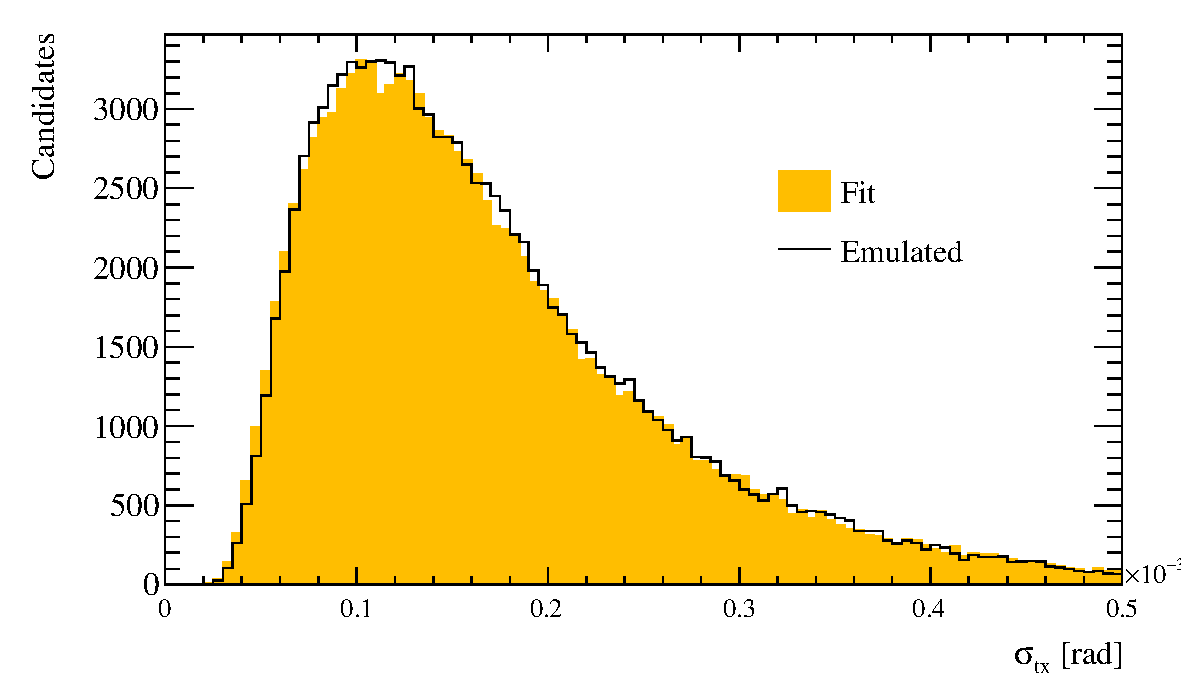
\includegraphics[width=0.48\textwidth]{figs/etx.pdf}
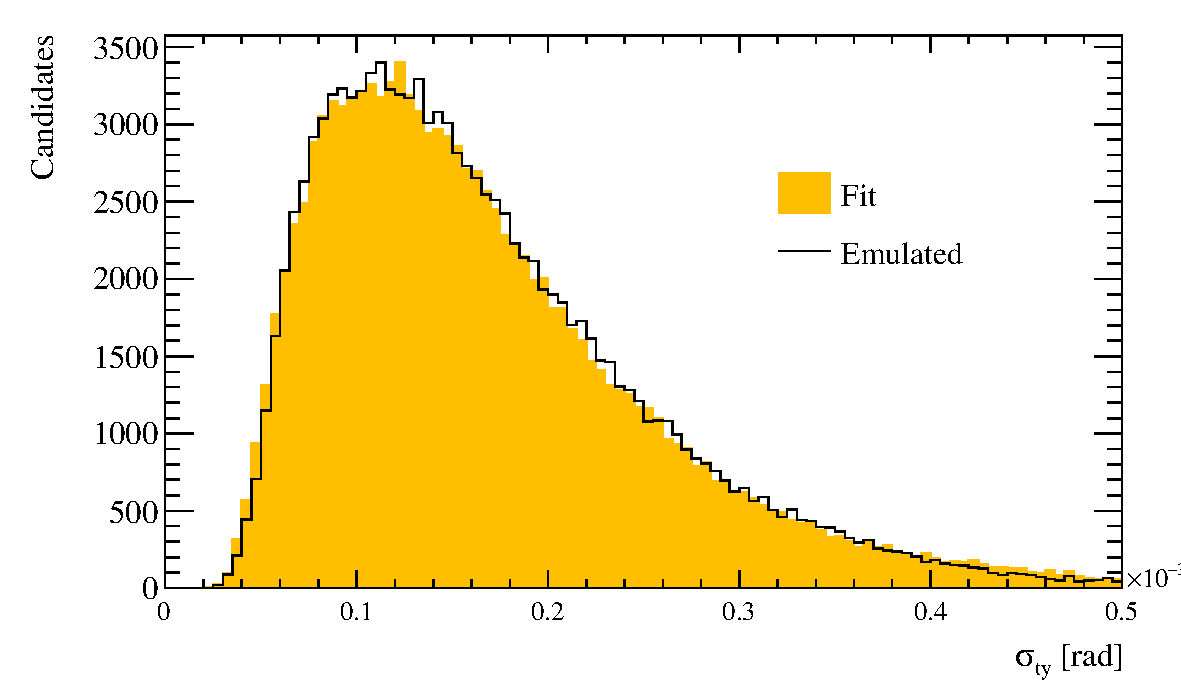
\includegraphics[width=0.48\textwidth]{figs/ety.pdf}
\caption{(Left)  Emulated and fit values of the uncertainty on $tx$
  and (Right) Emulated and fit values of the uncertainty on $ty$. }
\label{fig:etxty}
\end{figure}
%

%
The quality of the estimated uncertainties is judged from the
pulls. The RMS of this
distribution is 1.25. Fitting a double
Gaussian gives a central core with a width 0.91 and a wider Gaussian
with width 2. The fraction in the core is $90 \%$. It is easy to
incoporate these values into the emulator by using double Gaussian
smearing.  

An approach to emulating the uncertainties on $tx$ and $ty$ using a
parametric form was also developed but abandoned as it was found not
to work as well as the MVA approach. For completeness the results of
those studies are given in Appendix~\ref{sec:slopes}.